\chapter{Observations}
\label{chap:observations}

ADD IN WHAT IS ALMA PARAGRAPH HERE. What is a spectral window, etc with other jargon

Despite being a relatively young field, radio astronomy has provided crucial insights into many corners of the field of astronomy, ranging from making the first detections and characterizations of quasars, pulsars, and the Cosmic Microwave Background to observations of our own neighbors, including Jupiter and the Sun. Studying astronomical bodies, near or far, at radio frequencies allows astronomers to trace extremely low-energy emission and offers a chance to observe features that are simply invisible in other bands, like highly red-shifted galaxies or the extremely cold disks around young stars.

The very fact that observations at radio frequencies can be made at all is a testament to modern science. At long wavelengths, light behaves like a wave instead of as a particle, meaning that capturing that light requires a fundamentally different mindset than the intuitive photon-counting approach that optical and other shorter-wavelength astronomers can use. Furthermore, understanding these waves and their nature is a fundamentally recent achievement, one enabled by the revolution in physics of the early twentieth century.

The process of capturing and imaging these waves is a technical marvel in its own right, thanks to the marvels of inteferometry (described in \ref{section: interferometry})


\begin{figure}[b]
  \centering
  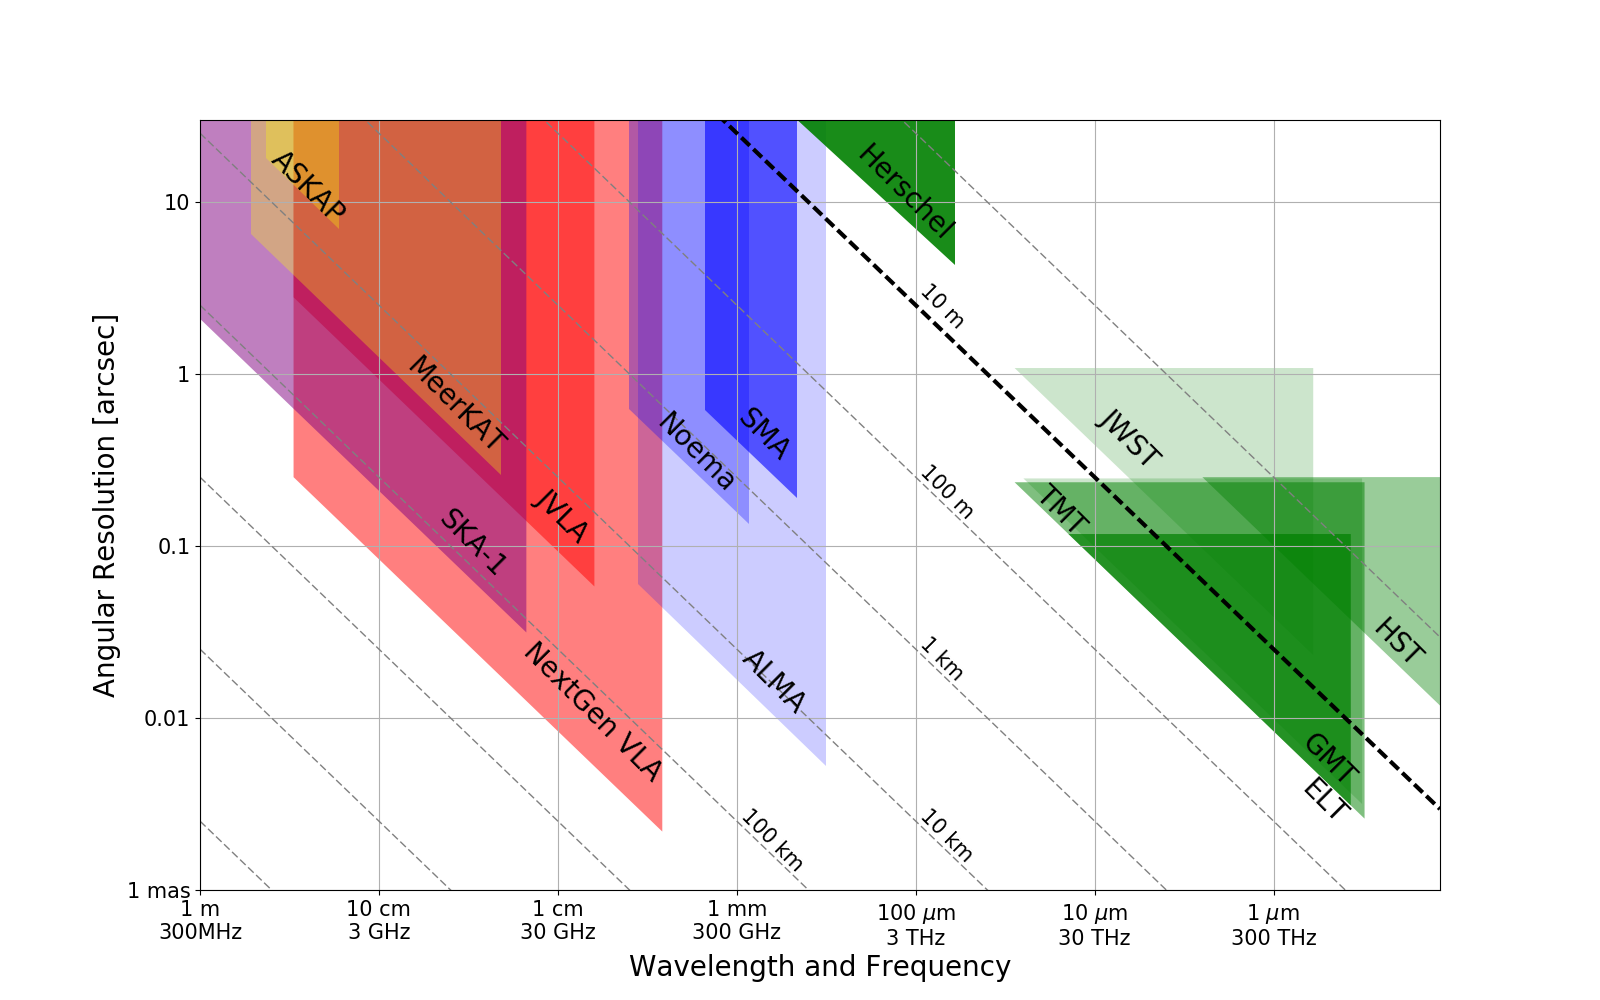
\includegraphics[width=\linewidth]{interferometers.png}
  \captionof{figure}{Current and future radio interferometers, contextualized by their blah}
  \label{fig:interferometers}
\end{figure}





The data presented in this thesis are part of an ALMA survey of Orion proplyds in Orion (project 2011.0.00028.S); data collection and analysis methods of the continuum results are presented in \citet{mann_alma_2014}. Since this was part of a Cycle 0 Early Science project, the survey used only 22 of the array's 50 12 meter dishes in a hybrid configuration, with baselines ranging from 21.2 to 384.2 meters, yielding maximum angular scales and angular resolution of 8" and 0."5, respectively. At a distance of 389 pc, max angular scales and angular resolution correspond to 3,112 AU and 194 AU, respectively. The distance to the stars used here was recently measured by Gaia (\citet{gaia_collaboration_gaia_2016}, \citet{gaia_collaboration_gaia_2018}) to be 389 $\pm$ 7.97, nearer than the previous measurement of 414 pc.
% sig figs on the distance
% For Gaia references: https://gea.esac.esa.int/archive/documentation/GDR2/bib.html#bib173
\bigskip

Observations were made on October 24, 2012, in ALMA's Band 7 receivers. Four spectral windows of width 1.875 GHz were arranged to cover the rest frequencies of the HCO+ (4-3), HCN (4-3), CO (3-2), and CS (7-6) transitions (356.734 GHz, 354.505 GHz, 345.796 GHz, and 342.883 GHz, respectively). Each band was split into 3840 channels with width 488.28 kHz, yielding a velocity resolution of 0.42 km s$^{-1}$.

\bigskip


Analysis showed that excluding baselines shorter than 110 k$\lambda$, 80 k$\lambda$, and 60 k$\lambda$ for HCO$^{+}$, HCN, and CO respectively optimized signal-to-noise ratios for each data set. The CS line showed no improvement with baseline cutting. See Section 3.1 for a more complete discussion of this process.


These data, from Field 4 of \citet{mann_alma_2014} represent 13.6 minutes of on-source time. This duration was split into six 136 second observations, spaced out over 7.5 hours to ensure adequate \textit{uv} coverage, yielding an RMS of 7mJy in the line data. The resulting synthesized beam has dimensions of of 0."57$\times$0."51 with a position angle of 85\degree. Precipitable water vapor in the atmosphere was stable at 0.7 mm.


The data were calibrated by ALMA staff using standard procedures in the Common Astronomy Software Applications (CASA, citation). The antenna-based complex gains and bandpass response of the system were calibrated using observations of the quasars J0607-085 and J0522-364 respectively. The absolute flux calibration was determined from observations of Callisto. The model of Callisto was drawn from Butler (2012) (citation). Absolute flux calibration is estimated to be accurate to within ∼ 10\% (\citet{mann_alma_2014}).

The velocity reference frame was converted from CASA's standard topocentric frame to LSRK (kinematic local standard of rest) using the CASA task \texttt{cvel}. Next, continuum emission was subtracted in the uv plane using the CASA task \texttt{contsub}. Visibilities were then inverted, deconvolved, and restored using standard procedures from the Multichannel Image Reconstruction Image Analysis and Display, or MIRIAD, package (\citet{rj_sault_astronomical_1995}).





% Note that no closing info is needed.
